\documentclass[border=3pt]{standalone}
\usepackage[T1]{fontenc}
\usepackage{lmodern}
\usepackage{amsmath,amssymb}
\usepackage{tikz}
\usetikzlibrary{arrows.meta,fit,backgrounds}

\definecolor{navy}{HTML}{1B2A4A}
\definecolor{brick}{HTML}{B81F28}
\definecolor{forest}{HTML}{2F5C44}
\definecolor{amber}{HTML}{F6D9B0}
\definecolor{warm}{HTML}{FDEADD}
\definecolor{mint}{HTML}{EAF2EC}
\definecolor{blush}{HTML}{FDECEC}
\definecolor{steel}{HTML}{E8EDF5}

\begin{document}
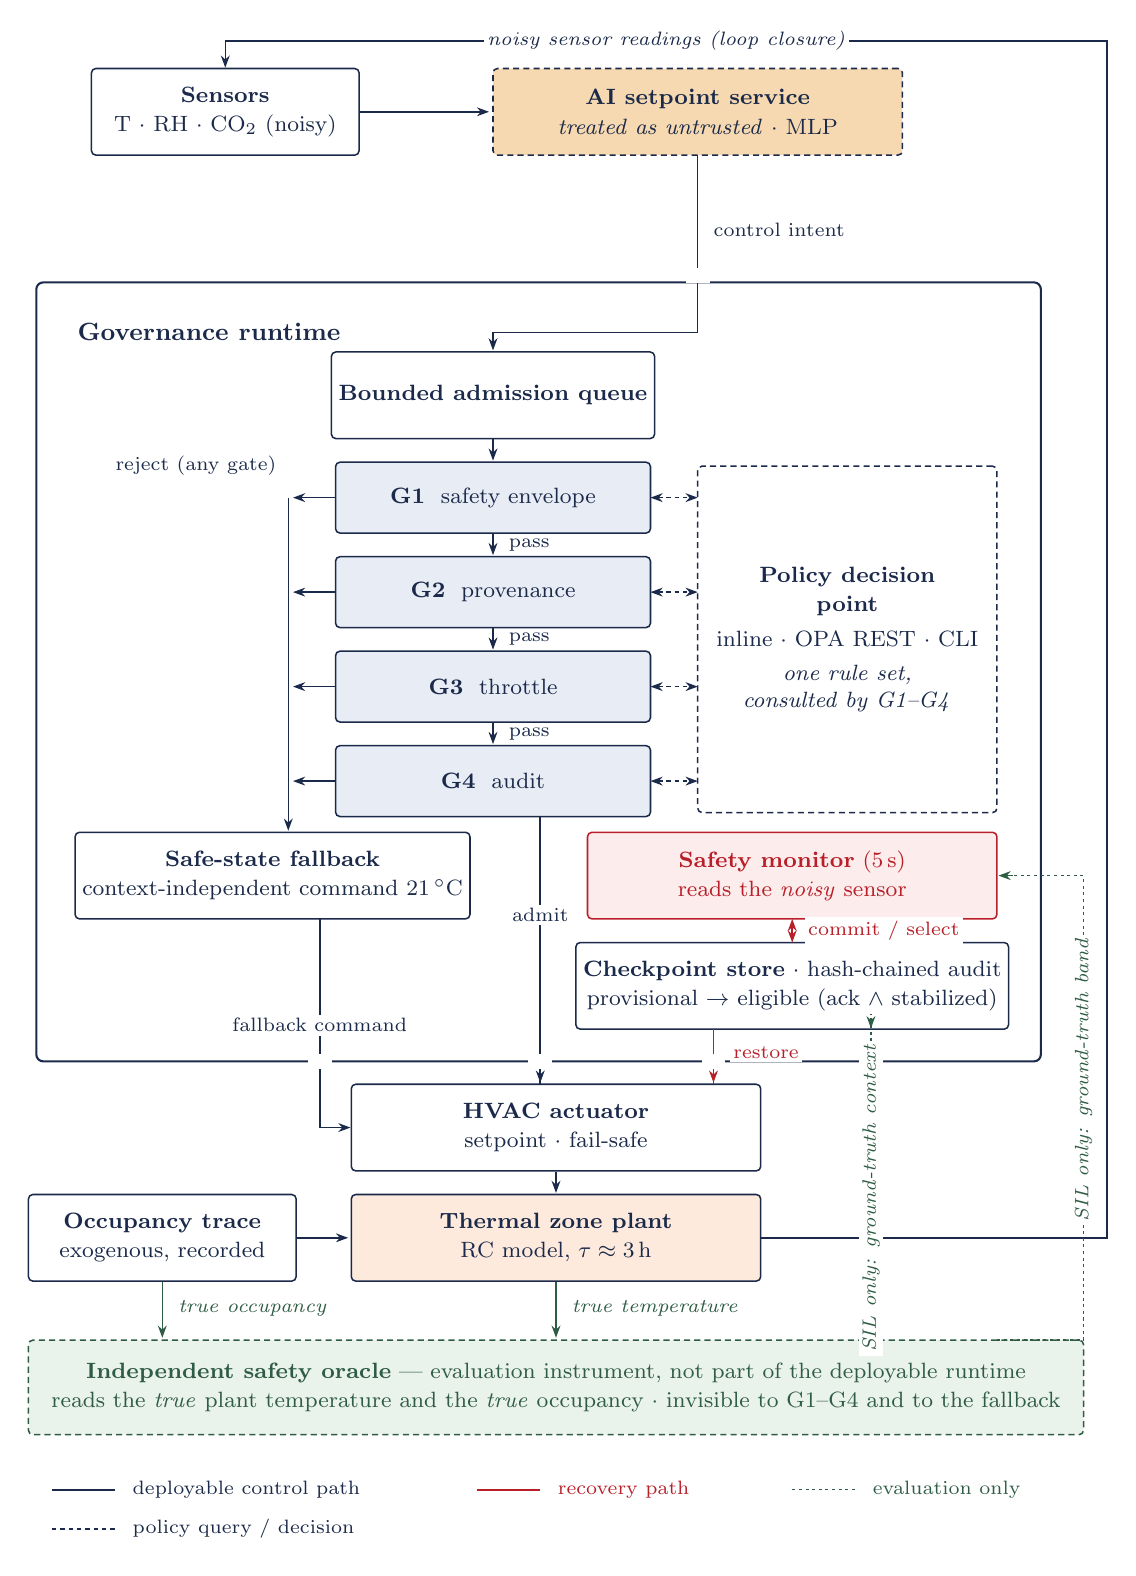
\begin{tikzpicture}[
  x=1mm, y=1mm, font=\footnotesize, text=navy,
  >={Stealth[length=4.4pt,width=3.2pt]},
  blk/.style   = {draw=navy, line width=.55pt, rounded corners=1.6pt, align=center,
                  inner sep=2.6pt, minimum height=11mm, fill=white, text=navy},
  gate/.style  = {blk, fill=steel, minimum height=9mm},
  ai/.style    = {blk, fill=amber, dashed, dash pattern=on 2.2pt off 1.5pt},
  pdp/.style   = {blk, dashed, dash pattern=on 2.2pt off 1.5pt},
  mon/.style   = {blk, draw=brick, fill=blush, text=brick},
  plant/.style = {blk, fill=warm},
  orc/.style   = {blk, draw=forest, fill=mint, text=forest, dashed,
                  dash pattern=on 2.2pt off 1.5pt},
  lbl/.style   = {font=\scriptsize, text=navy, inner sep=1.3pt, fill=white},
  rlbl/.style  = {font=\scriptsize, text=brick, inner sep=1.3pt, fill=white},
  glbl/.style  = {font=\scriptsize\itshape, text=forest, inner sep=1.3pt, fill=white},
  ln/.style    = {draw=navy, line width=.55pt},
  dl/.style    = {draw=navy, line width=.5pt, dash pattern=on 1.6pt off 1.4pt},
  rl/.style    = {draw=brick, line width=.6pt},
  gl/.style    = {draw=forest, line width=.5pt, dash pattern=on 1.1pt off 1.3pt},
  notch/.style = {fill=white, draw=none, inner sep=0pt, minimum width=3mm, minimum height=2mm},
]

% ---------------------------------------------------------------- sensing row
\node[blk, minimum width=34mm] (sens) at (28,148)
      {\textbf{Sensors}\\[1pt] T $\cdot$ RH $\cdot$ CO$_2$ (noisy)};
\node[ai, minimum width=52mm] (ai) at (88,148)
      {\textbf{AI setpoint service}\\[1pt] \emph{treated as untrusted} $\cdot$ MLP};
\draw[ln,->] (45,148) -- (61.5,148);

% ---------------------------------------------------------------- runtime interior
\node[font=\small\bfseries, text=navy, anchor=west] (title) at (8,120) {Governance runtime};

\node[blk, minimum width=34mm] (queue) at (62,112)
      {\textbf{Bounded admission queue}};
\node[gate, minimum width=40mm] (g1) at (62,99)  {\textbf{G1} \ safety envelope};
\node[gate, minimum width=40mm] (g2) at (62,87)  {\textbf{G2} \ provenance};
\node[gate, minimum width=40mm] (g3) at (62,75)  {\textbf{G3} \ throttle};
\node[gate, minimum width=40mm] (g4) at (62,63)  {\textbf{G4} \ audit};

\draw[ln,->] (62,106.5) -- (62,103.7);
\draw[ln,->] (62,94.5)  -- (62,91.7);
\draw[ln,->] (62,82.5)  -- (62,79.7);
\draw[ln,->] (62,70.5)  -- (62,67.7);
\node[lbl, anchor=west] at (63.5,93)  {pass};
\node[lbl, anchor=west] at (63.5,81)  {pass};
\node[lbl, anchor=west] at (63.5,69)  {pass};

% policy decision point, consulted by every gate
\node[pdp, minimum width=38mm, minimum height=44mm] (pdp) at (107,81)
      {\textbf{Policy decision}\\[1pt]\textbf{point}\\[3pt]
       inline $\cdot$ OPA REST $\cdot$ CLI\\[3pt]
       \emph{one rule set,}\\ \emph{consulted by G1--G4}};
\foreach \y in {99,87,75,63}{\draw[dl,<->] (82,\y) -- (88,\y);}

% reject rail
\foreach \y in {99,87,75,63}{\draw[ln,->] (42,\y) -- (36.6,\y);}
\draw[ln] (36,99) -- (36,58);
\draw[ln,->] (36,59) -- (36,56.7);
\node[lbl, anchor=east] at (35,103) {reject (any gate)};

\node[blk, minimum width=48mm] (fb) at (34,51)
      {\textbf{Safe-state fallback}\\[1pt] context-independent command 21\,$^\circ$C};

% monitor and checkpoint store
\node[mon, minimum width=52mm] (mo) at (100,51)
      {\textbf{Safety monitor} (5\,s)\\[1pt] reads the \emph{noisy} sensor};
\node[blk, minimum width=52mm] (ck) at (100,37)
      {\textbf{Checkpoint store} $\cdot$ hash-chained audit\\[1pt]
       provisional $\rightarrow$ eligible (ack $\wedge$ stabilized)};
\draw[rl,<->] (100,45.5) -- (100,42.5);
\node[rlbl, anchor=west] at (101.5,44) {commit / select};

% ---------------------------------------------------------------- frame
\begin{scope}[on background layer]
  \node[draw=navy, line width=.75pt, rounded corners=2.5pt, inner sep=4mm,
        fit=(title)(queue)(g4)(pdp)(fb)(ck)] (frame) {};
\end{scope}

% ---------------------------------------------------------------- plant column
\node[blk, minimum width=52mm] (act) at (70,19)
      {\textbf{HVAC actuator}\\[1pt] setpoint $\cdot$ fail-safe};
\node[plant, minimum width=52mm] (pl) at (70,5)
      {\textbf{Thermal zone plant}\\[1pt] RC model, $\tau\approx3$\,h};
\node[blk, minimum width=34mm] (occ) at (20,5)
      {\textbf{Occupancy trace}\\[1pt] exogenous, recorded};
\draw[ln,->] (70,13.4) -- (70,10.7);
\draw[ln,->] (37,5) -- (43.6,5);

% control intent into the queue
\draw[ln] (88,142.5) -- (88,120) -- (62,120);
\draw[ln,->] (62,120) -- (62,117.7);
\node[lbl, anchor=west] at (89.5,133) {control intent};

% admitted command
\draw[ln] (68,58.5) -- (68,24.5);
\draw[ln,->] (68,26) -- (68,24.7);
\node[lbl] at (68,46) {admit};

% fallback command
\draw[ln] (40,45.5) -- (40,19) -- (43.6,19);
\draw[ln,->] (42,19) -- (43.9,19);
\node[lbl] at (40,32) {fallback command};

% restore from an eligible checkpoint
\draw[rl] (90,31.5) -- (90,24.5);
\draw[rl,->] (90,26) -- (90,24.7);
\node[rlbl, anchor=west] at (92,28.5) {restore};

% loop closure
\draw[ln] (96,5) -- (140,5) -- (140,157) -- (28,157) -- (28,153.9);
\draw[ln,->] (28,155.4) -- (28,153.6);
\node[lbl] at (84,157) {\itshape noisy sensor readings (loop closure)};

% frame notches
\node[notch] at (88,127.2) {};
\node[notch] at (68,27.4) {};
\node[notch] at (40,27.4) {};
\node[notch] at (90,27.4) {};
\node[notch] at (110,27.4) {};
\node[notch, minimum width=2mm, minimum height=3mm] at (130.1,51) {};

% ---------------------------------------------------------------- oracle
\node[orc, minimum width=134mm, minimum height=12mm] (or) at (70,-14)
      {\textbf{Independent safety oracle} --- evaluation instrument, not part of the deployable runtime\\[1pt]
       reads the \emph{true} plant temperature and the \emph{true} occupancy $\cdot$ invisible to G1--G4 and to the fallback};
\draw[draw=forest, line width=.55pt,->] (70,-0.6) -- (70,-7.7);
\draw[draw=forest, line width=.55pt,->] (20,-0.6) -- (20,-7.7);
\node[glbl, anchor=west] at (71.5,-4) {true temperature};
\node[glbl, anchor=west] at (21.5,-4) {true occupancy};

% oracle -> checkpoint eligibility (SIL only)
\draw[gl] (110,-8) -- (110,33.4);
\draw[gl,->] (110,32) -- (110,31.6);
\node[glbl, rotate=90] at (110,10) {SIL only: ground-truth context};
% oracle -> monitor band selection (SIL only)
\draw[gl] (126,-8) -- (137,-8) -- (137,51) -- (126.4,51);
\draw[gl,->] (128,51) -- (126.2,51);
\node[glbl, rotate=90] at (137,25) {SIL only: ground-truth band};

% ---------------------------------------------------------------- legend
\draw[ln]  (6,-27) -- (14,-27);
\node[font=\scriptsize, text=navy,  anchor=west] at (15,-27) {deployable control path};
\draw[rl]  (60,-27) -- (68,-27);
\node[font=\scriptsize, text=brick, anchor=west] at (69,-27) {recovery path};
\draw[gl]  (100,-27) -- (108,-27);
\node[font=\scriptsize, text=forest, anchor=west] at (109,-27) {evaluation only};
\draw[dl]  (6,-32) -- (14,-32);
\node[font=\scriptsize, text=navy,  anchor=west] at (15,-32) {policy query / decision};

\end{tikzpicture}
\end{document}
